%% DONE USING OVERLEAF
%% PREAMBLE
\documentclass{beamer}       % Beamer is a class in LaTeX for presentations

\usetheme{Warsaw}            % theme and font theme affect the entire document
\usefonttheme{serif}
\usepackage[utf8]{inputenc}
\usepackage{hyperref}        % for \url{}
\usepackage{graphicx}
\usepackage{amsmath,mathtools}
\usepackage{xcolor}
\usepackage{enumitem} % necessary for enlarging max nesting limits
\usepackage{tikz} % required to make up for enumitem's incompatibility 

\makeatletter % required to allow use of the macros with '@' in them

% create beamer ball commands from scratch, since enumitem conflicts with beamer lists
\newcommand\beamerball{%
  \parbox[t]{10pt}{\raisebox{0.2pt}{\beamer@usesphere{item projected}{bigsphere}}}}

% tikzball to recreate the ball in enumerated lists, that 
\newcommand\tikzball[1]{%
    \tikz[baseline=(char.base)]{%
      \node[circle,ball color=blue!70!black, shade, color=white, inner sep=1.2pt] (char) {\tiny #1};
    }
}

% create new list for increased depth

\renewlist{itemize}{itemize}{6}
\setlist[itemize]{label=\beamerball, labelsep=0pt, leftmargin=2em}
\setlist[itemize, 1]{leftmargin=1.2em}
% necessary to specify to prevent negative labelwidth
\renewlist{enumerate}{enumerate}{6}
\setlist[enumerate]{label={\protect\tikzball{\arabic*}}, leftmargin=2em}
\setlist[enumerate, 1]{leftmargin=1.2em}

\makeatother

\title{Assignment-2}         % top matter
\subtitle{Software Systems Lab}
\author{\textit{B. Siddharth Prabhu}}
\institute{IIT Dharwad \\
\texttt{\href{mailto:200010003@iitdh.ac.in}{200010003@iitdh.ac.in}}
}
\date{August 15, 2021}
\titlegraphic{

\includegraphics[width=0.25\textwidth,height=0.25\textheight]{Image 2.jpeg}
}                            % scaling the given image down to fit

%% DOCUMENT BODY
\begin{document}

\begin{frame}
\maketitle                   % title frame
\end{frame}

%% \section{Dynamic Programming} %% commented out to prevent display on frame
\begin{frame}{Dynamic Programming}
\begin{itemize}              % itemized list
    \item Characteristics of Dynamic Programming
    \begin{enumerate}        % an enumerated list nested within
        \item \textit{Overlapping Sub-problems}
        \begin{block}{1}
        Subproblems are smaller versions of the original problem. Any problem has overlapping sub-problems if finding its solution involves solving the same subproblem multiple times.
        \end{block}
        \item \textit{Optimal Substructure}
        \begin{block}{2}
        Any problem has optimal substructure property if its overall optimal solution can be constructed from the optimal solutions of its subproblems.
        \end{block}
    \end{enumerate}
\end{itemize}
\end{frame}

%% \section{DP Methods}
\begin{frame}{DP Methods}
\begin{itemize}             % using \uncover<n->
    \uncover<1->{
    \item \textbf{Top-down with Memoization}
    \begin{block}{1}
    In this approach, we try to solve the bigger problem by recursively finding the solution to smaller sub-problems. Whenever we solve a sub-problem, we cache its result so that we don't end up solving it repeatedly if it's called multiple times. Instead, we can just return the saved result.
    \end{block}
    }
    \uncover<2->{
    \item \textbf{Bottom-up with Tabulation}
    \begin{alertblock}{2}   % alert block is red in color
    Tabulation is the opposite of the top-down approach and avoids recursion. In this approach, we solve the problem ``bottom-up'' (i.e. by solving all the related sub-problems first).
    \end{alertblock}
    }
\end{itemize}
\end{frame}

\begin{frame}[label=LABEL1]{Algorithms}
\setbeamercovered{transparent} % to lightly display covered contents of the frame
\begin{itemize}                % displaying itemized list item-by-item using \onslide
    \onslide<1-> \item Divide and Conquer
    \transsplitverticalin
    \onslide<2-> \item Greedy Algorithm
    \transsplitverticalin
    \onslide<3-> \item Dynamic Programming
    \transsplitverticalin
\end{itemize}
\end{frame}

\begin{frame}{Divide and Conquer}
\only<1>{                      % use of \only<n>
Example:\\ \textbf{Quick-Sort: The average case run time of quick sort is $O(n \ast log~n)$. This case happens when we don't exactly
get evenly balanced partitions.}
}
\only<2>{
\alert{Example:\\}              % \alert is used to highlight text
Merge Sort: \textcolor{orange}{The time complexity of Merge Sort is $O(n \ast log~n)$. \\ Merge Sort is useful for sorting linked lists in $O(n \ast log~n)$ time.}
}
\end{frame}

\begin{frame}{Hyperlinks}
\begin{itemize}                % placing buttons as items on a list, with hyperlinks
    \item \hyperlink{LABEL1}{Divide and Conquer}
    \item \hyperlink{LABEL1}{\beamergotobutton{Greedy Algorithm}}
    \item \hyperlink{LABEL1}{\beamerskipbutton{Dynamic Programming}}
\end{itemize}
\end{frame}

\begin{frame}{List of Data Structures}
\setbeamercovered{dynamic}     % lines are lighter, the later they are displayed
\begin{itemize}                % level 1
    \item<1-> Primitive
    \item<2-> Non-Primitive
    \begin{itemize}                % level 2
        \item<3-> \textit{Linear}
        \begin{itemize}                % level 3
            \item<4-> \textbf{Static}
            \begin{enumerate}             % level 4
                \item<5-> Array
            \end{enumerate}
            \item<4-> \textbf{Dynamic}
            \begin{enumerate}             % level 4
                \item<5-> Linked List
                \item<5-> Stack
                \item<5-> Queue
            \end{enumerate}
        \end{itemize}
        \item<6-> \textit{Non-Linear}
        \begin{enumerate}             % level 3
            \item<6-> Tree
            \item<6-> Graph
        \end{enumerate}
    \end{itemize}
\end{itemize}
\end{frame}

\begin{frame}{Data Structures}
\begin{figure}              % including graphics, similar to LaTeX articles
    \centering
    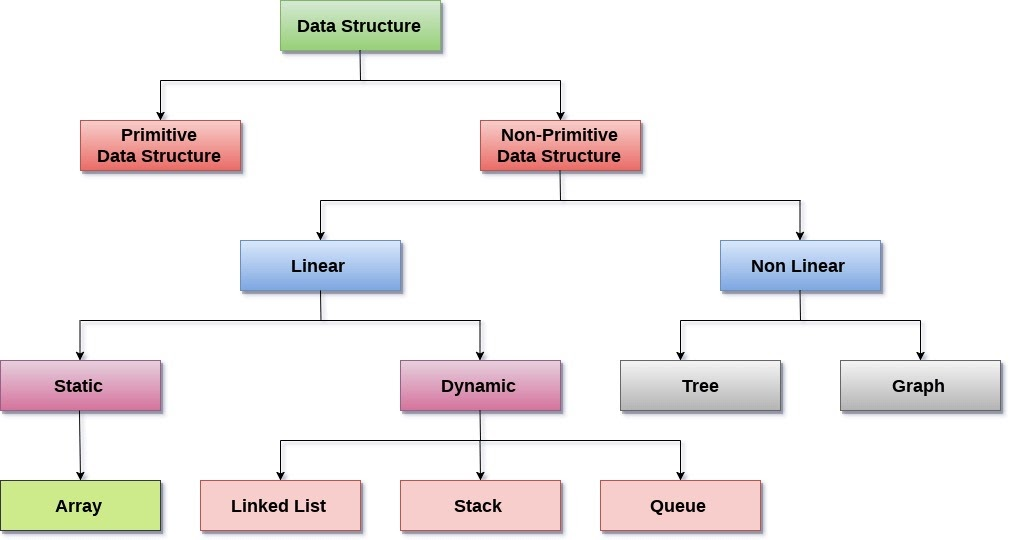
\includegraphics[scale=0.25]{Image 1.jpeg}
    \caption{1}
    \label{fig:fig_1}
\end{figure}
\end{frame}

\begin{frame}
    \begin{table}           % table display, similar to LaTeX articles
        \centering
        \begin{tabular}{|c|c|c|c|}
             \hline
             Algorithm & Best Case & Average Case & Worst Case  \\ 
             \hline \hline
             Linear Search & $O(1)$ & $O(n)$ & $O(n)$ \\
             \hline
             Binary Search & $O(1)$ & $O(log~n)$ & $O(log~n)$ \\
             \hline
             Bubble Sort & $O(n)$ & $O(n^2)$ & $O(n^2)$ \\
             \hline
             Selection Sort & $O(n^2)$ & $O(n^2)$ & $O(n^2)$ \\
             \hline
        \end{tabular}
        \caption{1}
        \label{tab:table1}
    \end{table}
    \begin{theorem}[Trigonometric Identity]
    $sin^2\theta + cos^2\theta = 1$
    \end{theorem}
\end{frame}

\begin{frame}
\begin{proof}               %% some math display
 Let a, b, c be lengths of right angled triangle.\\
\textbf{By definition,}
$$ sin\theta = b/c~\left(\frac{opposite~side}{hypotenuse}\right) $$
$$ cos\theta = a/c~\left(\frac{adjacent~side}{hypotenuse}\right) $$
$sin^2\theta + cos^2\theta = \frac{b^2}{c^2} + \frac{a^2}{c^2} = \frac{a^2 + b^2}{c^2}$ \\ \vspace{4mm}
\textbf{From Pythagoras' Theorem,} \\ \vspace{4mm}
$c^2 = a^2 + b^2$ \\ \vspace{4mm}
$\frac{a^2 + b^2}{c^2} = 1 \implies sin^2\theta + cos^2\theta = 1$ \\ \vspace{4mm}
\textbf{Hence, Proved.}
\end{proof}
\end{frame}

\begin{frame}{Multi-line Equations}  %% big equations that cause overfull hbox
     \begin{align*}
         f(x) = x^{6} + 7x^{3}y + 50x^{3}y^{2} &+ 12x^{2}y^{4} \\
         &- 19x^{5}y^{4} - 10x^{7}y^{6} + 7y^{4} - m^{3}n^{3}
     \end{align*} \pause   %% just to show that \pause works
     \begin{align*}
         \rho \Delta x \Delta y \Delta z \Delta \tau \partial_{t} c_{i}(t,x,\tau) 
         &= \rho \Delta x \Delta y \Delta z \Delta \tau (p_{i}-d_{i})  \\
         &- \rho \Delta y, \Delta z \Delta \tau [q_{i,x}(t,x + \Delta x/2, y, z, \tau)\\
         &\qquad - q_{i,x}(t,x - \Delta x/2, y, z, \tau)]\\
         &- \rho \Delta x, \Delta z \Delta  \tau [q_{i,y}(t,x,y+\Delta y/2, y, z, \tau)\\
         &\qquad - q_{i,y}(t,x,y - \Delta y/2, z, z, \tau)]\\
         &- \rho \Delta x \Delta y \Delta \tau[q_{i,z}(t,x,y,z + \Delta z/2, \tau) \\
         &\qquad - q_{i,z}(t,x,y,z-\Delta z/2, \tau)]
     \end{align*}
     %%Mathematical expression has been typed using subscripts and \qquad, which generates a 'double quadspace' to make it look like the aimed frames
\end{frame}
\end{document}
